\documentclass[letterpaper]{article}
\usepackage{settings}

\begin{document}
\begin{notes}{Part 1: Foundations and Image Filtering}

\NoteChapter{Foundations}

\NoteSection{Mathematical Representation of the Digital Image}

\textbf{Continuous Images.} One convenient mathematical model for an image is a real-valued function
$$f(x,y),$$
with $f: \R^2 \to \R$, where $x$, $y$ are spatial coordinates, and $f(x, y)$ is the intensity (brightness) at that point.\\

The function $f(x, y)$ is often modeled as the product of two components:
$$f(x, y) = i(x, y)r(x, y),$$
where
\begin{itemize}
    \item $i(x, y)$ is the illumination component, that is, the amount of source illumination incident on the scene being viewed, with $0\leq i(x,y) < \infty$
    \item $r(x, y)$ is the reflectance component, that is, the fraction of illumination reflected by the objects in the scene, with $0\leq r(x, y)\leq 1$
\end{itemize}
Reflectance is bounded by 0 (total absorption) and 1 (total reflection).


% \begin{figure}[H]
%     \centering
%     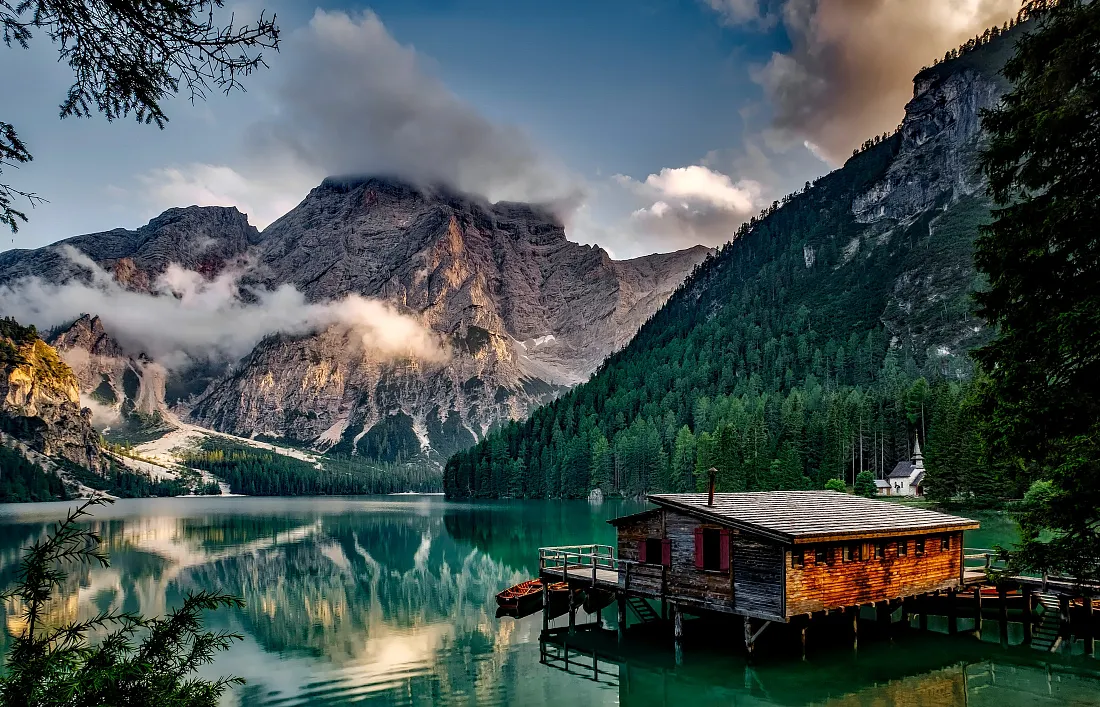
\includegraphics[width=0.7\linewidth]{images/part1/image.png}
% \end{figure}



\textbf{Discrete (Digital) Images.} A digital image is obtained by sampling the continuous image on a finite grid, so it becomes a discrete function or, equivalently, a matrix:
$$f(x, y) \in \R^{M\times N}.$$
Each entry in the matrix is a number, usually in $\{0,1,\dots,255\}$ for 8-bit images or in $[0,1]$ after normalization. Thus, a grayscale image is simply a 2D array of intensity values. For 16-bit images, the values range from 0 to 65,535, allowing smoother intensity gradients, less banding during editing, and better handling of high-dynamic-range (HDR) data.

\[
f(x,y) = 
\begin{bmatrix}
f(0, 0) & f(0, 1) & \cdots & f(0, N-1)\\
f(1, 0) & f(1, 1) & \cdots & f(1, N-1)\\
f(2, 0) & f(2, 1) & \cdots & f(2, N-1)\\
\vdots & \vdots & \ddots & \vdots\\
f(M-2, 0) & f(M-2, 1) & \cdots & f(M-2, N-1)\\
f(M-1, 0) & f(M-1, 1) & \cdots & f(M-1, N-1)\\
\end{bmatrix}
\]

For example, an image showing the letter D can be represented as
\begin{figure}[H]
    \centering
    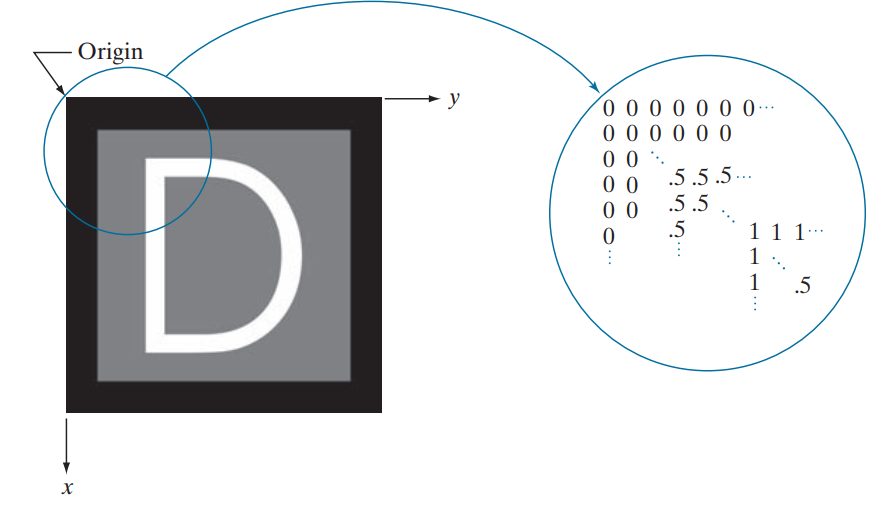
\includegraphics[width=0.7\linewidth]{images/part1/D_image.png}
\end{figure}
\noindent If the origin is at $(0,0)$ and the image indices run to $(M-1, N-1)$, then the center of an $M\times N$ digital image is
$$(x_c, y_c) = \left(\left\lfloor\frac{M}{2} \right\rfloor, \left\lfloor\frac{N}{2} \right\rfloor\right)$$


\textbf{Color Images (The RGB Model).} A color image extends the grayscale model by storing three channel values at every spatial location, one each for red, green, and blue:
$$f(x,y) = \bigl(f_R(x,y),\; f_G(x,y),\; f_B(x,y)\bigr) \in \R^{M\times N\times 3}.$$
Each channel $I_c \in \R^{M\times N}$ is itself a grayscale image, with values in $[0,255]$ (8-bit) or $[0,1]$ (normalized). The full image is therefore a 3D array (a \emph{tensor}) of shape $M\times N\times 3$. A pixel at $(x,y)$ is a 3-vector:
$$\mathbf{f}(x,y) = \begin{bmatrix}r \\ g \\ b\end{bmatrix}, \quad r,g,b \in [0,\,255].$$
The RGB model is \emph{additive}: $(0,0,0)$ is black and $(255,255,255)$ is white. Primary colors are $(255,0,0)$, $(0,255,0)$, $(0,0,255)$.


\begin{figure}[H]
    \centering
    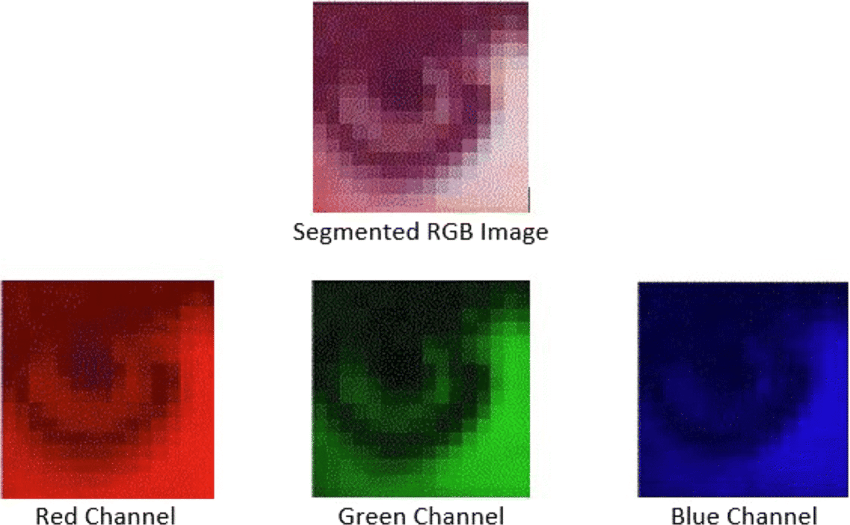
\includegraphics[width=0.7\linewidth]{images/part1/rgb-image.png}
    \caption{Any RGB image can be separated into red, green, and blue channels}
\end{figure}

\textbf{Color Images (The RGBA Model).} RGBA adds a fourth \emph{alpha} channel $\alpha\in[0,255]$ that encodes per-pixel opacity (transparency):
$$\mathbf{f}(x,y) = \bigl(f_R(x,y),\; f_G(x,y),\; f_B(x,y),\; f_A(x,y)\bigr) \in \R^{M\times N\times 4}.$$
$\alpha = 0$ means fully transparent; $\alpha = 255$ means fully opaque. When compositing a foreground image $\mathbf{F}$ over a background $\mathbf{B}$, the standard \emph{alpha compositing} formula (Porter–Duff ``over'' operator) is
$$\mathbf{C}(x,y) = \frac{\alpha}{255}\,\mathbf{F}(x,y) + \left(1 - \frac{\alpha}{255}\right)\mathbf{B}(x,y),$$
where the blend is applied independently to each of the R, G, and B channels.\\

\textbf{Multi-Channel and Hyperspectral Images.} The channel dimension is not limited to 3 or 4. In general, an image with $C$ channels is a tensor
$$\mathbf{f}(x,y) \in \R^{M\times N\times C},$$
where each channel records a different measurement at the same spatial location. Common examples:

\begin{itemize}
    \item \emph{RGB-D} ($C=4$): the fourth channel is a per-pixel \emph{depth} value (distance from the camera sensor) rather than transparency. Used in 3D reconstruction, robotics, and augmented reality (e.g.\ Microsoft Kinect, Intel RealSense).
    \item \emph{Multispectral} ($C \approx 4$–$15$): channels sample specific, non-overlapping spectral bands beyond visible light, typically including near-infrared (NIR) or thermal infrared. Common in satellite and aerial remote sensing (e.g.\ Landsat, Sentinel-2) for vegetation analysis (NDVI index), land-cover classification, and precision agriculture.
    \item \emph{Hyperspectral} ($C \approx 100$–$500$): hundreds of contiguous narrow spectral bands covering a wide range from UV to long-wave infrared. Each pixel is effectively a full reflectance spectrum, enabling material identification without physical contact. Applications include geological mineral mapping, food quality inspection, and surgical tissue classification.
    \item \emph{Medical volumetric images}: MRI and CT produce a stack of 2D slices, which can be treated as a 3D tensor $\R^{M\times N\times Z}$ (where $Z$ is the number of slices) or as multi-contrast images where each channel is a different acquisition sequence (T1, T2, FLAIR).
    \item \emph{Video frames}: a video clip is a 4D tensor $\R^{T\times M\times N\times 3}$, where $T$ is the number of frames and the channel dimension captures RGB color.
\end{itemize}

Processing high-channel images follows the same spatial principles as grayscale or RGB images, but the operations must also extend along the channel axis. For example, convolution filters are often applied channel-by-channel (or with 3D kernels), and distance metrics between pixels become vector norms in $\R^C$.



\columnbreaknofill

\NoteSection{Relationship Between Pixels}

\textbf{Neighborhood.} Let $p=(x,y)$ be a pixel with intensity $I(x,y)$.
The most common neighborhoods of $p$ are
\begin{itemize}
    \item $N_4(p)=\{(x+1,y), (x-1,y), (x,y+1), (x,y-1)\}$, the set of horizontal and vertical neighbors
    \item $N_D(p)=\{(x+1,y+1), (x+1,y-1), (x-1,y+1), (x-1,y-1)\}$, the set of diagonal neighbors
    \item $N_8(p)=N_4(p)\cup N_D(p)$, the full 8-neighborhood
\end{itemize}
These definitions apply only to neighbors that lie inside the image boundaries.

\begin{figure}[H]
    \centering
    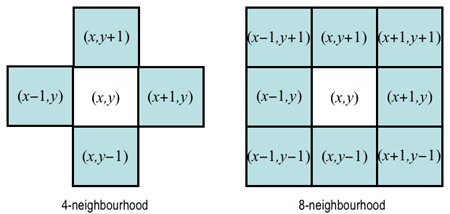
\includegraphics[width=0.6\linewidth]{images/part1/neighborhood.png}
\end{figure}


\textbf{Adjacency.} Let $V$ be a set of allowed gray levels, for example $V=\{1\}$ for binary images or $V=\{0,1,\dots,L-1\}$ for grayscale images.
Two pixels with values in $V$ are
\begin{itemize}
    \item \textbf{4-adjacent} if one pixel lies in the other pixel's $N_4$
    \item \textbf{8-adjacent} if one pixel lies in the other pixel's $N_8$
    \item \textbf{m-adjacent} if they are 4-adjacent, or if they are diagonal neighbors and their common 4-neighbors do not contain a pixel with value in $V$
\end{itemize}
Mixed adjacency avoids some of the ambiguity that occurs when diagonal connections create multiple possible paths.\\

\textbf{Path, Connectivity, Regions, and Boundaries.}
\begin{itemize}
    \item A \textit{path} from pixel $p$ to pixel $q$ is a sequence of distinct pixels $p_0, p_1, \dots, p_n$ such that $p_0=p$, $p_n=q$, and consecutive pixels are adjacent under the chosen adjacency rule.
    \item A set of pixels is \textit{connected} if there exists a path between any two pixels in the set.
    \item A \textit{region} is a connected set of pixels.
    \item The \textit{boundary} of a region consists of the pixels in the region that have at least one neighbor outside the region.
\end{itemize}

\textbf{Distance Measures.} For pixels $p=(x,y)$ and $q=(s,t)$, common distance measures are
\begin{align*}
    D_E(p,q) &= \sqrt{(x-s)^2 + (y-t)^2} && \text{(Euclidean distance)}\\
    D_4(p,q) &= |x-s| + |y-t| && \text{(city-block distance)}\\
    D_8(p,q) &= \max(|x-s|, |y-t|) && \text{(chessboard distance)}
\end{align*}
The set of pixels at distance 1 from $p$ under $D_4$ is exactly $N_4(p)$, and under $D_8$ is exactly $N_8(p)$.

\NoteSection{Tools used in Digital Image Processing}

\textbf{Hadamard Product.} For matrices $A,B\in\R^{m\times n}$ of the same size, the Hadamard product is the elementwise product

$$A \odot B$$

with entries
$$
(A\odot B)_{ij} = A_{ij}B_{ij}.
$$
Unlike matrix multiplication, the Hadamard product multiplies corresponding pixels directly and is commonly used for masking and pointwise weighting.\\

\textbf{Kernel (Mask / Filter).} A kernel is a small matrix that specifies how to combine a pixel with its neighbors. Sliding a kernel across an image produces a new image whose value at each location depends on a local neighborhood.\\

\textbf{Weighted Sum.} Many image processing operations compute the output pixel as a weighted sum of neighboring pixels:
$$
g(x,y) = \sum_m \sum_n w(m,n)f(x-m,y-n)
$$
where $w(m,n)$ are the kernel weights. Smoothing, sharpening, and edge detection can all be expressed this way.\\

\textbf{Convolution.} For an image $f$ and kernel $h$, the 2D convolution is
$$
(f*h)(x,y) = \sum_m \sum_n f(m,n)h(x-m, y-n).
$$
Convolution combines nearby pixels using a shifted and flipped version of the kernel. It is the fundamental operation behind many spatial filters.\\

\textbf{Correlation.} The 2D correlation of $f$ with kernel $h$ is
$$
(f\star h)(x,y) = \sum_m \sum_n f(x+m, y+n)h(m,n).
$$
Correlation looks similar to convolution, but the kernel is not flipped. In practice, many software libraries implement filtering in a way that is closer to correlation.\\

\textbf{Separable Kernels.} A 2D kernel is separable if it can be written as the outer product of two 1D kernels:
$$
h(x,y)=a(x)b(y).
$$
Then a 2D filtering operation can be performed as two 1D passes, which reduces computation and storage. Gaussian smoothing is a standard example.


\NoteSection{Operations on Images}

Operations on images fall into four broad categories based on how many pixels from the input image contribute to each output pixel.

\begin{enumerate}
    \item \textit{Point (Pixel) Operations}: output depends only on the single corresponding input pixel, $g(x,y) = T(f(x,y))$.
    \item \textit{Local (Neighborhood) Operations}: output depends on a small window around the pixel, $g(x,y) = T(f(x',y') : (x',y')\in W_{x,y})$.
    \item \textit{Global Operations}: output at every pixel depends on \emph{all} input pixels (e.g.\ Fourier transform, histogram equalization).
    \item \textit{Geometric Operations}: the spatial arrangement of pixels is altered (translation, rotation, scaling) without necessarily changing their values.
\end{enumerate}

\textbf{Arithmetic Operations.} Given two same-size images $f$ and $g$, arithmetic operations are applied element-wise:

\begin{itemize}
    \item \textit{Addition}: $(f+g)(x,y)=f(x,y)+g(x,y)$. Averaging $k$ noisy versions of the same scene,
    $$\bar{f}(x,y) = \frac{1}{k}\sum_{i=1}^k f_i(x,y),$$
    reduces zero-mean noise: the standard deviation of the noise decreases as $1/\sqrt{k}$.

    \item \textit{Subtraction}: $(f-g)(x,y)=f(x,y)-g(x,y)$. Difference images highlight regions that changed between two acquisitions. Mask-mode radiography subtracts a pre-injection image from a post-injection image to reveal blood vessels.

    \item \textit{Multiplication}: $(f\cdot g)(x,y)=f(x,y)\cdot g(x,y)$. Multiplying by a binary mask sets selected regions to zero (region-of-interest extraction). Shading correction divides by a flat-field image to compensate for non-uniform illumination.

    \item \textit{Division}: $(f/g)(x,y)=f(x,y)/g(x,y)$ (where $g\neq 0$). Used in flat-field correction and ratio imaging.
\end{itemize}

Results are typically clamped to $[0, L-1]$ or normalized after the operation to prevent overflow or underflow.\\

\textbf{Logical (Set) Operations.} For binary images with pixel values in $\{0,1\}$, the standard Boolean operations apply element-wise:

\begin{align*}
    \text{NOT: } & \bar{f}(x,y) = 1 - f(x,y)\\
    \text{AND: } & (f\wedge g)(x,y) = f(x,y)\cdot g(x,y)\\
    \text{OR: }  & (f\vee g)(x,y)   = \min(f(x,y)+g(x,y),1)\\
    \text{XOR: } & (f\oplus g)(x,y) = |f(x,y)-g(x,y)|
\end{align*}

For 8-bit gray-scale images these become bitwise operations on the 8-bit representations of each pixel. AND is used for masking, OR for combining regions, XOR for detecting differences, and NOT for image complementing (equivalent to the image negative $s=(L-1)-r$).\\

\textbf{Geometric (Spatial) Operations.} A geometric operation maps every pixel $(x,y)$ in the output to a location $(x',y')$ in the input via a spatial transformation $T$:
$$(x',y') = T(x,y).$$
The output pixel value is then obtained by interpolating the input at the (generally non-integer) location $(x',y')$. Common interpolation methods are nearest-neighbor, bilinear, and bicubic. Important geometric transforms include translation, rotation, scaling, and affine and perspective transforms — treated in Chapter 2.


\newpage


\NoteChapter{Image Transformation}

\NoteSection{2D Systems}


A \textbf{2D system} (or image operator) $S$ maps an input image $f(x,y)$ to an output image $g(x,y)$:
$$g(x,y) = S[f(x,y)].$$
The most important class is \textbf{linear shift-invariant (LSI)} systems, whose output is always expressible as a 2D convolution with an impulse response.\\

\textbf{Properties of 2D Systems.}
\begin{enumerate}
    \item \textit{Linearity.} $S$ is linear if superposition holds for all constants $a$, $b$ and images $f_1$, $f_2$:
    $$S[af_1(x,y) + bf_2(x,y)] = a\,S[f_1(x,y)] + b\,S[f_2(x,y)].$$
    Every kernel-based filter (smoothing, sharpening, edge detection) is linear. Histogram equalization and morphological operations are \emph{not} linear.

    \item \textit{Shift-Invariance (Space-Invariance).} $S$ is shift-invariant if shifting the input shifts the output by the same amount:
    $$S[f(x-x_0,\, y-y_0)] = g(x-x_0,\, y-y_0).$$
    A filter applied to a corner of the image behaves identically to the same filter applied to the center. Vignetting corrections and spatially adaptive filters break shift-invariance.

    \item \textit{Linearity + Shift-Invariance $\Rightarrow$ Convolution.} If $S$ is both linear and shift-invariant, then there exists a unique \textbf{impulse response} $h(x,y)$ such that
    $$g(x,y) = (f * h)(x,y) = \sum_m\sum_n f(m,n)\,h(x-m,\,y-n).$$
    This is the fundamental theorem of LSI systems: the entire behavior is captured by $h$.

    \item \textit{Stability (BIBO).} $S$ is bounded-input, bounded-output stable if every bounded input produces a bounded output:
    $$\sup_{x,y}|f(x,y)| < \infty \;\Rightarrow\; \sup_{x,y}|g(x,y)| < \infty.$$
    For an LSI system, BIBO stability is equivalent to $h$ being absolutely summable: $\sum_{x,y}|h(x,y)| < \infty$. All finite-support kernels (e.g.\ Gaussian blur, Sobel) are stable.

    \item \textit{Locality.} $S$ is \textbf{local} if each output pixel $g(x,y)$ depends on only a finite neighborhood of $(x,y)$ in the input. Convolution with a finite kernel is local. Global operations such as histogram equalization or the Fourier transform are \textbf{non-local} because $g(x,y)$ depends on all pixels of $f$.

    \item \textit{Memoryless (Pointwise).} A special case of locality: $g(x,y)$ depends only on $f(x,y)$ itself, not on any neighbors. All intensity transformations $g = T(f)$ (log, gamma, negation) are memoryless.

    \item \textit{Invertibility.} $S$ is invertible if there exists an inverse system $S^{-1}$ that perfectly recovers the input:
    $$S^{-1}[S[f(x,y)]] = f(x,y).$$
    For an LSI system with impulse response $h$, invertibility means $H(u,v) \neq 0$ for all $(u,v)$, so the inverse filter $H^{-1}(u,v)=1/H(u,v)$ exists. In practice, near-zero values of $H$ amplify noise, motivating regularized inverses (Wiener filter).
\end{enumerate}





\NoteSection{Intensity Transformation}

A \textbf{spatial domain} operation is applied directly to image pixels. For a digital image $f(x,y)$ with gray levels in $[0, L-1]$ (where $L=256$ for 8-bit images), any such operation can be written as
$$
g(x,y) = T\bigl[f(x,y)\bigr],
$$
where $T$ is an operator defined over some neighborhood of $(x,y)$. When $T$ operates on a $1\times 1$ neighborhood, it depends only on the intensity at that pixel and is called a \textbf{point} (intensity) \textbf{transformation}:
$$
s = T(r),\quad r,s\in[0,L-1],
$$
where $r$ is the input gray level and $s$ is the output gray level. When $T$ uses a wider neighborhood it becomes \textbf{spatial filtering}.

\NoteSubsection{Basic Intensity Transformations}

\textbf{Identity.} $s = r$. The output is identical to the input; used as a baseline reference.\\

\textbf{Image Negative.} Reverses the intensity scale:
$$s = (L-1) - r.$$
Dark regions become bright and vice versa. Useful for enhancing detail embedded in dark areas, and equivalent to a photographic negative.

\begin{figure}[H]
    \centering
    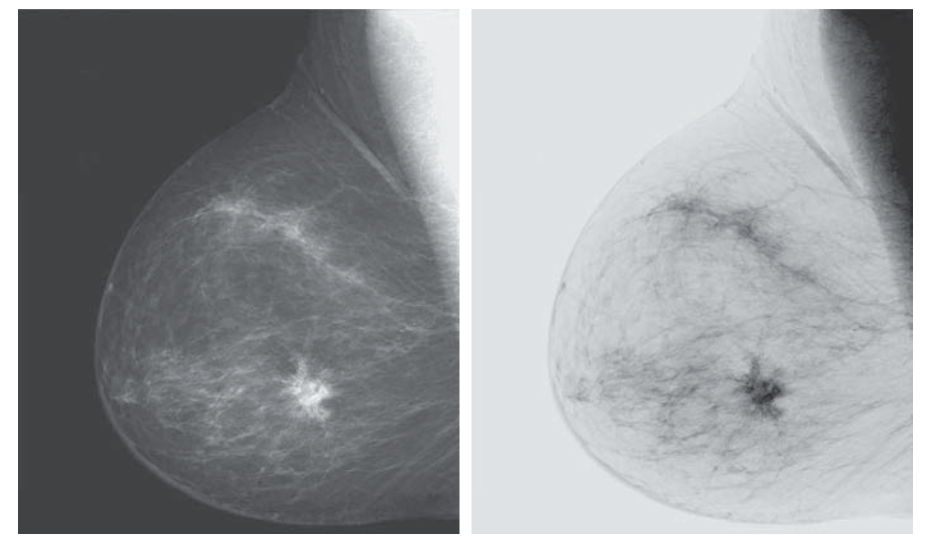
\includegraphics[width=0.75\linewidth]{images/part1/image-negative.png}
\end{figure}

\textbf{Log Transformation.} Compresses a wide dynamic range into a displayable range:
$$s = c\log(1 + r),$$
where $c = (L-1)/\log(1 + r_{\max})$ normalizes the output to $[0,L-1]$. Low gray levels are expanded and high gray levels are compressed, making it ideal for displaying Fourier spectra whose magnitude spans many decades.\\

\textbf{Inverse Log (Exponential) Transformation.} The opposite of the log transform:
$$s = c\bigl(e^{r} - 1\bigr).$$
High gray levels are expanded more than low gray levels. Useful when detail is concentrated in bright regions.\\

\textbf{Power-Law (Gamma) Transformation.}
$$s = c\,r^{\gamma},\quad c>0,\;\gamma>0.$$
\begin{itemize}
    \item $0 < \gamma < 1$: brightens the image (expands dark tones)
    \item $\gamma > 1$: darkens the image (expands bright tones)
    \item $\gamma = 1$, $c=1$: identity
\end{itemize}
\textbf{Gamma correction} compensates for the nonlinear $\gamma\approx 2.2$ response of display devices. Cameras apply an encoding gamma $\gamma_{\text{enc}}\approx 1/2.2$ so that the round-trip from scene to screen is approximately linear.

\NoteSubsection{Piecewise-Linear Transformations}

Many practical transformations are built from connected line segments, which makes them easy to design and interpret.

\textbf{Contrast Stretching.} Linearly maps an input range $[r_{\min}, r_{\max}]$ to the full output range $[0, L-1]$:
$$
s = \frac{r - r_{\min}}{r_{\max} - r_{\min}}\,(L-1).
$$
If the original image is low-contrast and occupies only a narrow band of intensities, this stretches that band to fill $[0, L-1]$. A more flexible form uses two breakpoints $(r_1, s_1)$ and $(r_2, s_2)$:
$$
s = \begin{cases}
\dfrac{s_1}{r_1}\,r, & 0 \le r < r_1,\\[6pt]
s_1 + \dfrac{s_2-s_1}{r_2-r_1}(r-r_1), & r_1 \le r < r_2,\\[6pt]
s_2 + \dfrac{(L-1)-s_2}{(L-1)-r_2}(r-r_2), & r_2 \le r \le L-1.
\end{cases}
$$

\textbf{Thresholding.} A special case of contrast stretching with infinite slope at $r=T$:
$$
s = \begin{cases}
0, & r < T,\\
L-1, & r \ge T.
\end{cases}
$$
Produces a binary image; the fundamental operation in segmentation.

\textbf{Gray-Level Slicing.} Highlights a band $[A,B]$ of intensities.
\begin{itemize}
    \item \emph{Binary mode}: $s = L-1$ for $A\le r\le B$, else $s=0$ (background suppressed).
    \item \emph{Preserve mode}: $s = L-1$ for $A\le r\le B$, else $s=r$ (background kept). Useful for isolating objects of a particular brightness without losing context.
\end{itemize}

\textbf{Bit-Plane Slicing.} Each pixel in an 8-bit image decomposes as
$$
r = \sum_{k=0}^{7} b_k \, 2^k, \quad b_k\in\{0,1\}.
$$
The $k$-th bit plane is the binary image formed by extracting $b_k$ from every pixel. Higher bit planes (MSBs) carry the dominant structure; lower planes carry fine detail and noise. Bit-plane reconstruction with only the top few planes gives a compressed approximation of the original.

\NoteSubsection{Histogram Processing}

The \textbf{histogram} of an image counts how often each gray level occurs:
$$
h(r_k) = n_k, \quad k = 0, 1, \dots, L-1,
$$
where $n_k$ is the number of pixels with gray level $r_k$ and the total pixel count is $n = \sum_k n_k$. The normalized histogram $p(r_k) = n_k/n$ estimates the probability density of the intensity levels.\\

\textbf{Histogram Equalization.} Automatically spreads intensity levels to produce a nearly uniform histogram, maximizing contrast. The transformation is the cumulative distribution function (CDF) of the input histogram:
$$
s_k = T(r_k) = (L-1)\sum_{j=0}^{k} p(r_j) = \frac{(L-1)}{n}\sum_{j=0}^{k} n_j.
$$
Properties:
\begin{itemize}
    \item Monotonically increasing, so it preserves the ordering of gray levels
    \item No free parameters; fully automatic
    \item Tends to over-enhance low-contrast images by amplifying noise in flat regions
\end{itemize}

\textbf{Histogram Matching (Specification).} Instead of targeting a uniform output histogram, a desired output distribution $p_z(z)$ is specified. The procedure:
\begin{enumerate}
    \item Equalize the input: $s = T(r)$ using the input CDF.
    \item Compute the CDF $G(z)$ of the desired distribution.
    \item Apply the inverse map: $z = G^{-1}(s) = G^{-1}(T(r))$.
\end{enumerate}
This generalizes histogram equalization and is useful when a reference image with the desired tonal character is available.





\columnbreaknofill


\NoteChapter{Convolution Operator and the Fourier Transform}

\NoteSection{The 2D Convolution Operation}

For a small discrete kernel, each output pixel is obtained by placing the kernel center at $(x,y)$, multiplying corresponding entries, and summing the results. So convolution replaces each pixel by a weighted combination of its neighbors.

For a $3\times 3$ kernel $h$, this can be written as
$$
g(x,y)= h(x, y) * f(x, y) = \sum_{m=-1}^{1}\sum_{n=-1}^{1} h(m,n)f(m-x,n-y).
$$

\textbf{Why it matters.}
\begin{itemize}
    \item If the kernel coefficients are nonnegative and sum to 1, convolution performs smoothing or averaging
    \item If the kernel emphasizes differences between neighbors, convolution can sharpen edges or detect boundaries
    \item Many imaging systems are modeled as linear shift-invariant systems, and convolution is the natural operation for such systems
\end{itemize}

\textbf{Important facts.}
\begin{itemize}
    \item The kernel is flipped in both coordinates before multiplication
    \item The output size near the image border depends on the boundary rule used, such as zero padding, replication, or reflection
    \item Convolution is linear and commutative: $f*h = h*f$
\end{itemize}

\textbf{Common examples.}
An averaging (or box) filter can be written as
$$
\frac{1}{9}
\begin{bmatrix}
1 & 1 & 1\\
1 & 1 & 1\\
1 & 1 & 1
\end{bmatrix}
$$
which blurs the image by replacing each pixel with the local average. A discrete Laplacian-type kernel such as
$$
\begin{bmatrix}
0 & -1 & 0\\
-1 & 4 & -1\\
0 & -1 & 0
\end{bmatrix}
$$
emphasizes rapid intensity changes and is therefore useful for edge detection and sharpening.

\NoteSubsection{Properties of 2D Convolution}

Let $f$, $g$, $h$ be images/signals and $a$, $b$ be scalars.

\begin{enumerate}
    \item \textit{Commutativity.} $$f * h = h * f$$
    \item \textit{Associativity.} $$(f * g) * h = f * (g * h)$$
    \item \textit{Distributivity.} $$f * (g + h) = f * g + f * h$$
    \item \textit{Linearity.} $$f * (ag + bh) = a(f * g) + b(f * h)$$
    \item \textit{Shift-Invariance.}
    If $g(x,y) = (f * h)(x,y)$, then a spatial shift of the input by $(x_0, y_0)$ produces the same shift in the output:
    $$f(x - x_0,\, y - y_0) * h(x,y) = g(x - x_0,\, y - y_0).$$
    This means the response of the system looks the same regardless of where in the image it is applied.
    \item \textit{Separability.} A kernel $h(x,y)$ is \textbf{separable} if it can be written as
    $$h(x,y) = h_1(x)\, h_2(y).$$
    In that case the 2D convolution reduces to two sequential 1D convolutions:
    $$f * h = (f *_x h_1) *_y h_2,$$
    reducing complexity from $O(MN\,k^2)$ to $O(MN\,k)$ for a $k\times k$ kernel. The Gaussian kernel is the canonical separable example:
    \begin{align*}
        G_\sigma(x,y) &= \frac{1}{2\pi\sigma^2}e^{-(x^2+y^2)/(2\sigma^2)}\\ 
        &= \left(\frac{1}{\sqrt{2\pi}\,\sigma}e^{-x^2/(2\sigma^2)}\right)\left(\frac{1}{\sqrt{2\pi}\,\sigma}e^{-y^2/(2\sigma^2)}\right)
    \end{align*}

    \item \textit{Derivative Property.}
    $$\frac{\partial}{\partial x}(f * h) = \left(\frac{\partial f}{\partial x}\right) * h = f * \left(\frac{\partial h}{\partial x}\right).$$
    Differentiation commutes with convolution, so edge-detection derivatives can be precomputed into the kernel.
\end{enumerate}









\textbf{Convolution Theorem.}
Convolution in the spatial domain is equivalent to pointwise multiplication in the frequency domain:
$$\mathcal{F}\{f * h\} = \mathcal{F}\{f\} \cdot \mathcal{F}\{h\}.$$
This is one of the most important results in signal processing: a large kernel can be applied to a large image efficiently via two FFTs and an elementwise product, rather than direct summation.



\NoteSubsection{Boundary Handling}

Because the kernel extends beyond the image at the borders, a boundary rule must be chosen:
\begin{itemize}
    \item \textbf{Zero padding} - pixels outside the image are treated as 0; common default but introduces dark border artifacts.
    \item \textbf{Replication (clamp)} - the nearest border pixel value is repeated; avoids dark halos.
    \item \textbf{Reflection} - pixel values are mirrored across the border; preserves smooth appearance near edges.
    \item \textbf{Circular (wrap)} - the image is assumed periodic; consistent with frequency-domain (FFT-based) convolution.
\end{itemize}
The choice affects output pixels only within $\lfloor k/2\rfloor$ of the image border for a $k\times k$ kernel.




\NoteSection{The 2D Fourier Transform}

\NoteSubsection{Continuous 2D Fourier Transform}

The \textbf{2D Fourier Transform} of a continuous image $f(x,y)$ is defined as
$$F(u,v) = \int_{-\infty}^{\infty}\int_{-\infty}^{\infty} f(x,y)\, e^{-j2\pi(ux+vy)}\, dx\, dy,$$
where $u$ and $v$ are spatial-frequency coordinates (cycles per unit length). The \textbf{inverse} recovers the original image:
$$f(x,y) = \int_{-\infty}^{\infty}\int_{-\infty}^{\infty} F(u,v)\, e^{j2\pi(ux+vy)}\, du\, dv.$$
Together these form a transform pair, written $f(x,y) \xleftrightarrow{\;\mathcal{F}\;} F(u,v)$.

\NoteSubsection{Discrete 2D Fourier Transform (DFT)}

For an $M\times N$ digital image $f(x,y)$ with $x\in\{0,\dots,M-1\}$ and $y\in\{0,\dots,N-1\}$, the \textbf{2D DFT} is
$$F(u,v) = \sum_{x=0}^{M-1}\sum_{y=0}^{N-1} f(x,y)\, e^{-j2\pi\!\left(\frac{ux}{M}+\frac{vy}{N}\right)},$$
for $u\in\{0,\dots,M-1\}$, $v\in\{0,\dots,N-1\}$. The \textbf{inverse DFT} is
$$f(x,y) = \frac{1}{MN}\sum_{u=0}^{M-1}\sum_{v=0}^{N-1} F(u,v)\, e^{j2\pi\!\left(\frac{ux}{M}+\frac{vy}{N}\right)}.$$

\textbf{Separability of the DFT.}
The 2D DFT is separable: it can be computed as $N$ 1D DFTs along rows followed by $M$ 1D DFTs along columns (or vice versa). Using the FFT algorithm, the total cost is $O(MN\log MN)$.\\


\textbf{Algorithms.} The FFT computes the DFT in $O(N\log N)$ instead of $O(N^2)$ by exploiting the \emph{Cooley--Tukey} divide-and-conquer structure. The 2D FFT reduces to repeated 1D FFTs via separability.

\begin{itemize}
    \item \textbf{The 1D Cooley--Tukey FFT (radix-2).} For a length-$N = 2^k$ sequence $f[x]$, split it into even- and odd-indexed halves and apply the \emph{butterfly} recursion. Let $W_N = e^{-j2\pi/N}$ be the primitive $N$-th root of unity. Then
    $$F[u] = \underbrace{\sum_{x=0}^{N/2-1} f[2x]\,W_{N/2}^{ux}}_{F_{\mathrm{even}}[u]} + W_N^u \underbrace{\sum_{x=0}^{N/2-1} f[2x+1]\,W_{N/2}^{ux}}_{F_{\mathrm{odd}}[u]},$$
    and using the periodicity $F_{\mathrm{even}}[u + N/2] = F_{\mathrm{even}}[u]$:
    \begin{align*}
    F[u]       &= F_{\mathrm{even}}[u] + W_N^u\,F_{\mathrm{odd}}[u], \\
    F[u+N/2]   &= F_{\mathrm{even}}[u] - W_N^u\,F_{\mathrm{odd}}[u].
    \end{align*}
    Each butterfly combines two values with one complex multiply and two additions. Applying recursively yields $\log_2 N$ stages of $N/2$ butterflies each: total $O(N\log N)$ operations.
    
    \item\textbf{2D FFT via row-column decomposition.}
    \begin{enumerate}
        \item Apply the 1D FFT to each of the $M$ rows of $f(x,y)$, producing an intermediate array $F_{\mathrm{row}}(x,v)$:
        $$F_{\mathrm{row}}(x,v) = \sum_{y=0}^{N-1} f(x,y)\,e^{-j2\pi vy/N}, \quad v=0,\dots,N-1.$$
        Cost: $M$ transforms of length $N$ $\Rightarrow$ $O(MN\log N)$.
        \item Apply the 1D FFT to each of the $N$ columns of $F_{\mathrm{row}}$, producing $F(u,v)$:
        $$F(u,v) = \sum_{x=0}^{M-1} F_{\mathrm{row}}(x,v)\,e^{-j2\pi ux/M}, \quad u=0,\dots,M-1.$$
        Cost: $N$ transforms of length $M$ $\Rightarrow$ $O(MN\log M)$.
    \end{enumerate}
    Total cost: $O(MN\log M + MN\log N) = O(MN\log MN)$. For a square $N\times N$ image this is $O(N^2 \log N)$, compared to $O(N^4)$ for naive 2D DFT.
\end{itemize}



\textbf{Notes.}
\begin{itemize}
    \item \emph{Zero-padding to a power of 2} (or products of small primes) enables the radix-2 FFT and avoids wrap-around artifacts when the image size is not $2^k$.
    \item \emph{fftshift}: the raw FFT output places DC at index $(0,0)$ (top-left). Calling \texttt{fftshift} cyclically shifts the array so DC appears at the center $(M/2,N/2)$, making the spectrum easier to visualise and filter.
    \item For real-valued images, conjugate symmetry $F(-u,-v)=F^*(u,v)$ means only half the spectrum is independent; the \emph{real FFT} (RFFT) exploits this to halve computation and storage.
    \item Frequency-domain filtering: compute $G = H\cdot F$, then $g = \mathcal{F}^{-1}\{G\}$. Faster than direct convolution for kernels larger than $\approx 9\times9$ on a $512\times512$ image.
\end{itemize}


\NoteSubsection{Spectrum, Phase, and Power}

Any complex-valued $F(u,v) = R(u,v) + j I(u,v)$ can be written in polar form:
\begin{align*}
    |F(u,v)| &= \sqrt{R^2 + I^2} && \text{(magnitude / amplitude spectrum)}\\
    \angle F(u,v) &= \arctan\!\left(\frac{I}{R}\right) && \text{(phase spectrum)}\\
    |F(u,v)|^2 &= R^2 + I^2 && \text{(power spectrum)}
\end{align*}
The \textbf{magnitude} encodes which frequencies are present and how strongly; the \textbf{phase} encodes where features are located in space. For natural images, most energy concentrates near the origin (low frequencies), where the DC component $F(0,0) = \sum_{x,y} f(x,y)$ equals the total intensity sum.

\NoteSubsection{Properties of the 2D DFT}

Let $f(x,y)\xleftrightarrow{\mathcal{F}} F(u,v)$ and $g(x,y)\xleftrightarrow{\mathcal{F}} G(u,v)$.

\begin{enumerate}
    \item \textit{Linearity.}
    $$af(x,y) + bg(x,y) \;\xleftrightarrow{\mathcal{F}}\; aF(u,v) + bG(u,v).$$
    
    \item \textit{Translation (Shift Theorem).}
    $$f(x-x_0,\, y-y_0) \;\xleftrightarrow{\mathcal{F}}\; F(u,v)\, e^{-j2\pi(ux_0/M \,+\, vy_0/N)}.$$
    A spatial shift introduces a linear phase ramp in the frequency domain but does not change the magnitude spectrum.
    
    \item \textit{Modulation (Frequency Shift).}
    $$f(x,y)\, e^{j2\pi(u_0x/M \,+\, v_0y/N)} \;\xleftrightarrow{\mathcal{F}}\; F(u-u_0,\, v-v_0).$$
    Multiplying by a complex exponential shifts the spectrum. In particular, multiplying $f(x,y)$ by $(-1)^{x+y}$ shifts the zero-frequency component to the center of the DFT array (the standard \emph{fftshift} operation).
    
    \item \textit{Conjugate Symmetry (Real Images).}
    If $f(x,y)$ is real-valued, then
    $$F(-u,-v) = F^*(u,v),$$
    meaning the spectrum is conjugate-symmetric. Therefore, only half the DFT coefficients are independent.
    
    \item \textit{Convolution Theorem.}
    $$f(x,y) * h(x,y) \;\xleftrightarrow{\mathcal{F}}\; F(u,v)\cdot H(u,v).$$
    Spatial convolution becomes elementwise multiplication in the frequency domain.
    
    \item \textit{Correlation Theorem.}
    $$f(x,y)\star h(x,y) \;\xleftrightarrow{\mathcal{F}}\; F^*(u,v)\cdot H(u,v).$$
    Cross-correlation in the spatial domain corresponds to complex-conjugate multiplication in frequency.
    
    \item \textit{Parseval's (Energy) Theorem.}
    $$\sum_{x=0}^{M-1}\sum_{y=0}^{N-1}|f(x,y)|^2 = \frac{1}{MN}\sum_{u=0}^{M-1}\sum_{v=0}^{N-1}|F(u,v)|^2.$$
    Total signal energy is preserved (up to scaling) by the DFT.
    
    \item \textit{Rotation.}
    If $f(x,y)$ is rotated by angle $\theta$, then $F(u,v)$ rotates by the same $\theta$. Circular structures in space therefore produce circular structures in the spectrum.
    
    \textit{Scaling.}
    $$f(ax, by) \;\xleftrightarrow{\mathcal{F}}\; \frac{1}{|ab|}F\!\left(\frac{u}{a},\frac{v}{b}\right).$$
    Compression in space produces expansion in frequency (the uncertainty principle for images).
\end{enumerate}



\NoteSubsection{Periodicity of the DFT}

The 2D DFT implicitly treats the image as a periodic tile repeated infinitely. Both $F(u,v)$ and the recovered $f(x,y)$ are periodic with periods $M$ and $N$:
$$F(u+M,\, v) = F(u,\, v+N) = F(u,v).$$
This periodicity causes the \textbf{wrap-around} artifact: objects near one border interact with the opposite border when a frequency-domain filter is applied. Zero-padding to a larger array before the FFT mitigates this effect.


\NoteSubsection{Common Transform Pairs}

\begin{center}
\begin{tabular}{@{}ll@{}}
\toprule
Spatial domain $f(x,y)$ & Frequency domain $F(u,v)$ \\
\midrule
$\delta(x,y)$ (impulse) & $1$ (constant) \\
$1$ (constant) & $\delta(u,v)$ \\
$e^{j2\pi(u_0x/M+v_0y/N)}$ & $\delta(u-u_0,v-v_0)$ \\
$\cos\bigl(2\pi(u_0x/M+v_0y/N)\bigr)$ & $\tfrac{1}{2}[\delta(u\!-\!u_0,v\!-\!v_0)+\delta(u\!+\!u_0,v\!+\!v_0)]$ \\
$\text{rect}(x,y)$ (box) & $\text{sinc}(u)\,\text{sinc}(v)$ \\
$e^{-(x^2+y^2)/(2\sigma^2)}$ (Gaussian) & $2\pi\sigma^2 e^{-2\pi^2\sigma^2(u^2+v^2)}$ (Gaussian) \\
\bottomrule
\end{tabular}
\end{center}


\columnbreaknofill

\NoteChapter{Spatial-Domain Image Filtering}

\NoteSection{Linear Filtering}

Spatial filtering applies a kernel $h$ to an image $f$ by sliding it across every pixel and computing a weighted sum of the local neighborhood. The output at $(x,y)$ is

$$g(x,y) = \sum_{i=-a}^{a}\sum_{j=-b}^{b} h(i,j)\,f(x-i,\,y-j),$$

for a kernel of size $(2a+1)\times(2b+1)$. This is correlation (no flip); for convolution, replace $f(x+s, y+t)$ with $f(x-s, y-t)$. For symmetric kernels the two are identical.\\

\textbf{Smoothing (Low-Pass) Filters.} Attenuate high-frequency detail (noise, texture) and retain low-frequency structure.

\begin{enumerate}
    \item \textit{Box Filter (Averaging).} Replaces each pixel with the mean of its $k\times k$ neighborhood:
    $$h_{\text{box}}(x,y) = \frac{1}{k^2}\begin{bmatrix}1&1&\cdots&1\\\vdots&&\ddots&\vdots\\1&1&\cdots&1\end{bmatrix}.$$
    Fast and simple, but blurs edges and introduces ringing on sharp transitions because the box function's Fourier transform is a sinc with slowly decaying side-lobes.\\
    
    \item \textit{Gaussian Filter.} Uses a Gaussian-shaped kernel:
    
    $$h(x,y)=G_\sigma(x,y) = \frac{1}{2\pi\sigma^2}e^{-(x^2+y^2)/(2\sigma^2)}.$$
    
    $\sigma$ controls the spread: larger $\sigma$ gives stronger smoothing. The Gaussian is the optimal smoothing filter in the sense that it minimizes the joint uncertainty in space and frequency (Heisenberg-like tradeoff). It produces no ringing because its Fourier transform is also Gaussian. The kernel is separable, so it can be implemented as two 1D passes: cost $O(MNk)$ vs.\ $O(MNk^2)$ for a non-separable kernel.
\end{enumerate}


\NoteSection{Non-linear Filtering}

\begin{enumerate}
    \item \textit{Median Filter (Nonlinear).} Replaces each pixel with the \emph{median} of its neighborhood rather than the mean. Nonlinear - cannot be expressed as a convolution. Key property: it removes \emph{impulse noise} (salt-and-pepper) without blurring edges, because the median is robust to outliers. The mean, by contrast, averages in the spike value and spreads it to neighbors.

    \item \textit{Bilateral Filter (Nonlinear).} A filter that Reduces the noise and Preserves the edges. Commonly known as the equation

    $$g(\mathbf{x}) = BF[f]_p= \frac{1}{W_p}\sum_{q\in S}G_{\sigma_s}\left( \Vert p -q \Vert \right)G_{\sigma_r}\left(|f_p - f_q|\right)f_q$$

    or,
    
    $$g(x,y) = \frac{1}{W_p}\sum_{s}\sum_{t}G_{\sigma_s}(s,t)\,G_{\sigma_r}\!\bigl(f(x+s,y+t)-f(x,y)\bigr)f(x+s,y+t)\,$$
    
    where $G_{\sigma_s}$ is the spatial Gaussian (penalises distant pixels), $G_{\sigma_r}$ is the range Gaussian (penalises pixels with very different intensity), and $W_p$ is a normalisation constant. 

    $$W_p=\sum_{q\in S}G_{\sigma_s}\left( \Vert p -q \Vert \right)G_{\sigma_r}\left(|I_p - I_q|\right)$$
    
    Pixels across a strong edge have large intensity difference, so $G_{\sigma_r}\approx 0$ and they do not contribute - the edge is preserved. $\sigma_s$ controls the spatial smoothing radius; $\sigma_r$ controls sensitivity to intensity differences. Nonlinear and non-convolution; more expensive than Gaussian filtering.

    \item \textit{Anisotropic Diffusion (Perona--Malik, Nonlinear).} A PDE-based filter that iteratively smooths an image while suppressing diffusion across edges. The evolution equation is
    $$\frac{\partial f}{\partial t} = \mathrm{div}\!\bigl[c(|\nabla f|)\,\nabla f\bigr],$$
    where the diffusion coefficient $c$ is a decreasing function of the gradient magnitude, e.g.\ $c(|\nabla f|)=e^{-(|\nabla f|/K)^2}$. Where $|\nabla f|$ is small (flat region), $c\approx 1$ and diffusion is isotropic; where $|\nabla f|$ is large (edge), $c\approx 0$ and diffusion stops. Each time step is one iteration of smoothing; more steps give stronger smoothing. The result is a \emph{cartoon-like} image: piecewise-smooth regions with crisp boundaries.
\end{enumerate}


\NoteSection{High-pass (Sharpening) Filters}

Amplify high-frequency detail - edges, fine texture - to enhance apparent sharpness.

\begin{enumerate}
    \item \textit{Laplacian Sharpening.} The discrete Laplacian measures the second-order spatial derivative:
    $$\nabla^2 f = \frac{\partial^2 f}{\partial x^2} + \frac{\partial^2 f}{\partial y^2} \approx f(x+1,y)+f(x-1,y)+f(x,y+1)+f(x,y-1)-4f(x,y),$$
    giving the $4$-connected kernel (and an $8$-connected version that includes diagonals):
    $$h_L = \begin{bmatrix}0&1&0\\1&-4&1\\0&1&0\end{bmatrix}, \qquad h_L' = \begin{bmatrix}1&1&1\\1&-8&1\\1&1&1\end{bmatrix}.$$
    The Laplacian responds to intensity changes in \emph{all directions}, making it isotropic. To sharpen, add the Laplacian back to the original (noting sign convention - use $+$ if center coefficient is negative, $-$ if positive):
    $$g(x,y) = f(x,y) - \nabla^2 f(x,y).$$
    This can be done in one step with the composite kernel $h = \delta - h_L$.
    
    \item \textit{Unsharp Masking.} Subtracts a blurred (low-pass) version of the image to obtain a high-pass residual, then adds it back:
    $$g = f + k\,(f - f_{\text{blur}}) = (1+k)f - k\,f_{\text{blur}},$$
    where $k>0$ controls sharpening strength and $f_{\text{blur}} = f * G_\sigma$. When $k=1$ this is standard unsharp masking; $k>1$ is called \emph{high-boost filtering}. The mask $f - f_{\text{blur}}$ is the unsharp mask - it contains only the edges and fine detail absent from the blurred image.
\end{enumerate}



\textbf{Gradient-Based Edge Detection.} Edges correspond to rapid intensity changes, detected by large first-order derivatives.

\begin{enumerate}
    \item \textit{Gradient.} The image gradient at $(x,y)$ is the vector
    $$\nabla f = \begin{bmatrix}\partial f/\partial x \\ \partial f/\partial y\end{bmatrix},$$
    with \emph{magnitude} $|\nabla f| = \sqrt{(\partial f/\partial x)^2 + (\partial f/\partial y)^2}$ and \emph{direction} $\theta = \arctan(\partial f/\partial y,\; \partial f/\partial x)$. Large magnitude $\Rightarrow$ edge; direction $\perp$ the edge orientation.
    
    \item \textit{Sobel Operator.} Approximates the gradient with $3\times3$ kernels that simultaneously smooth perpendicular to the derivative direction (reducing noise sensitivity):
    $$h_x = \begin{bmatrix}-1&0&1\\-2&0&2\\-1&0&1\end{bmatrix}, \qquad h_y = \begin{bmatrix}-1&-2&-1\\0&0&0\\1&2&1\end{bmatrix}.$$
    $G_x = f * h_x$ and $G_y = f * h_y$ approximate $\partial f/\partial x$ and $\partial f/\partial y$.\\

    \textbf{Why these weights?} Each kernel is \emph{separable}: it factors into a 1D derivative filter crossed with a 1D smoothing filter applied in the perpendicular direction:
    $$h_x \;=\; \underbrace{\begin{bmatrix}1\\2\\1\end{bmatrix}}_{\text{smooth in }y} \otimes \underbrace{\begin{bmatrix}-1 & 0 & 1\end{bmatrix}}_{\text{diff.\ in }x}.$$
    \begin{itemize}
        \item \textbf{Row $[-1,\,0,\,1]$:} central-difference approximation of $\partial/\partial x$, computing $f(x{+}1)-f(x{-}1)$. The center weight is $0$ because the central pixel cancels in the symmetric difference.
        \item \textbf{Column $[1,\,2,\,1]^T$:} binomial smoothing in $y$ (perpendicular to the derivative). These are the degree-2 binomial coefficients $\binom{2}{k}$, the discrete analog of a Gaussian. Smoothing \emph{across} the edge suppresses noise without blurring the edge response in $x$, since a step edge is already constant along its length.
        \item \textbf{Why not uniform $[1,1,1]^T$?} A box average has a sinc-shaped frequency response with slow-decaying side-lobes that let high-frequency noise leak through. The binomial $[1,2,1]$ more closely approximates the Gaussian (which has no side-lobes), giving stronger noise rejection. The heavier center weight $2$ acts like the Gaussian peak.
    \end{itemize}

    \item \textit{The Prewitt Operator.} Same separable structure as Sobel, but uses \emph{uniform} averaging $[1,1,1]^T$ instead of binomial smoothing:
    $$h_x \;=\; \underbrace{\begin{bmatrix}1\\1\\1\end{bmatrix}}_{\text{box avg.\ in }y} \otimes \underbrace{\begin{bmatrix}-1 & 0 & 1\end{bmatrix}}_{\text{diff.\ in }x} = \begin{bmatrix}-1&0&1\\-1&0&1\\-1&0&1\end{bmatrix},  $$
    $$h_y = \begin{bmatrix}-1&-1&-1\\0&0&0\\1&1&1\end{bmatrix}.$$
    All three rows receive equal weight. This is simpler to interpret - the gradient is just the difference of top and bottom row averages - but less noise-robust than Sobel: the flat box filter passes more high-frequency noise than Sobel's Gaussian-weighted rows. Sobel is the more common default for this reason.

    \item \textit{Robinson Compass Operator.} While Sobel and Prewitt estimate only two orthogonal gradient components ($x$ and $y$), the Robinson operator detects edges in \emph{eight compass directions} - N, NE, E, SE, S, SW, W, NW - using eight $3\times3$ kernels generated by cyclically rotating a single template. The north kernel and its east neighbor are:
    $$K_N = \begin{bmatrix}-1&-1&-1\\0&0&0\\1&1&1\end{bmatrix}, \qquad K_{NE} = \begin{bmatrix}-1&-1&0\\-1&0&1\\0&1&1\end{bmatrix}.$$
    All eight kernels are obtained by rotating $K_N$ in $45^\circ$ steps (equivalently, rotating the $3\times3$ grid of coefficients). Each kernel uses the values $\{-1, 0, 1\}$ with the same \emph{three-level} pattern, so it shares the uniform-averaging character of Prewitt (no Gaussian weighting). The edge strength in each direction $d$ is $R_d = K_d * f$; the overall response is
    $$|\nabla f|_{\text{Robinson}} = \max_{d}\,|R_d|,$$
    and the dominant direction $d^*$ gives the estimated edge orientation.

    \textbf{Why eight directions?} Sobel and Prewitt reconstruct gradient direction from $(G_x, G_y)$ assuming the derivative is well-approximated along the two axis-aligned directions. The Robinson operator instead directly measures responses along all $45^\circ$-spaced axes, which gives a more accurate magnitude estimate for edges that run diagonally (at $45^\circ$), where the axis-aligned kernels underestimate the gradient. The trade-off is eight convolutions instead of two.
    
    \item \textit{Laplacian of Gaussian (LoG).} Combines Gaussian smoothing with the Laplacian to detect edges robustly:
    $$\text{LoG}(x,y) = \nabla^2\bigl[G_\sigma * f\bigr] = \bigl(\nabla^2 G_\sigma\bigr) * f.$$
    The LoG kernel has a characteristic ``Mexican hat'' shape. Edge locations are found at the \emph{zero-crossings} of the LoG response (where the second derivative changes sign). By the convolution theorem, $\nabla^2 G_\sigma$ can be precomputed as a single kernel.
\end{enumerate}


\NoteSection{Kernel Construction}


\newpage

\NoteChapter{Frequency-Domain Filtering}

Frequency-domain filtering exploits the convolution theorem: instead of sliding a kernel over the image, multiply the image spectrum $F$ by a transfer function $H$ pointwise and invert. All filter distances below are measured from the shifted spectrum center: 
$$D(u,v)=\sqrt{(u-M/2)^2+(v-N/2)^2}$$

\textbf{Workflow.}
\begin{enumerate}
    \item Pad $f$ to $(M+k-1)\times(N+k-1)$ to prevent circular wrap-around.
    \item Compute $F=\mathcal{F}\{f\}$.
    \item Form $H(u,v)$.
    \item Multiply $G = H \cdot F$.
    \item Invert $g = \mathcal{F}^{-1}\{G\}$ and crop.
\end{enumerate}
Direct convolution costs $O(MNk^2)$; this pipeline costs $O(MN\log MN)$ regardless of kernel size, with crossover near $k\approx 9$ for $512\times512$. Composing two filters is free: apply $H_1 H_2$ in one FFT pair.\\

\textbf{Low-Pass Filters (smoothing / noise removal).}

\begin{enumerate}
    \item \textit{Ideal LPF.} $H = \mathbf{1}[D \le D_0]$: a hard disk in frequency. All components outside radius $D_0$ are zeroed. Simple but causes severe \emph{ringing} (Gibbs phenomenon) - a sharp circular window in frequency corresponds to a jinc-ripple impulse response in space.

    \item \textit{Butterworth LPF} (order $n$).
    $$H(u,v) = \frac{1}{1+(D/D_0)^{2n}}.$$
    Smooth, monotone rolloff that eliminates ringing. Higher $n$ gives a steeper transition approaching the ideal. $n=2$ is a common practical choice.

    \item \textit{Gaussian LPF.}
    $$H(u,v) = e^{-D^2/(2\sigma^2)}.$$
    No ringing, since the Fourier transform of a Gaussian is another Gaussian. Equivalent to Gaussian spatial filtering and is the preferred default when no ringing can be tolerated.

 
\end{enumerate}

\textbf{High-Pass Filters (edge enhancement / sharpening).} Any low-pass $H_{\text{LP}}$ gives a complementary high-pass:
$$H_{\text{HP}}(u,v) = 1 - H_{\text{LP}}(u,v).$$
Ideal HPF rings for the same reason as ideal LPF; Butterworth and Gaussian HPFs do not. High-pass filtering zeros the DC component ($F(0,0)$) and amplifies edges and fine detail.\\

\textbf{Band-Pass, Band-Reject, and Notch Filters.}

\begin{enumerate}
    \item \textit{Band-pass / band-reject.} A band-pass selects frequencies in an annulus $[D_{\text{low}}, D_{\text{high}}]$:
    $$H_{\text{BP}} = H_{\text{HP},D_{\text{low}}} \cdot H_{\text{LP},D_{\text{high}}}.$$
    Band-reject ($H_{\text{BR}} = 1 - H_{\text{BP}}$) suppresses the same ring, useful for removing periodic textural noise at a known spatial frequency.
    
    \item \textit{Notch filter.} Zeros isolated frequency pairs $\pm(u_0, v_0)$ that correspond to periodic noise (scan lines, moiré patterns). These appear as bright symmetric spots in $|F(u,v)|$ and are most naturally removed by placing small reject disks at those locations.
\end{enumerate}



\textbf{Homomorphic Filtering (illumination correction).} Exploits $f = i \cdot r$. The log linearises the product:
$$\ln f = \ln i + \ln r.$$
A high-pass-like transfer function then suppresses low-frequency illumination ($\gamma_L < 1$) while boosting high-frequency reflectance detail ($\gamma_H > 1$):
$$H(u,v) = (\gamma_H - \gamma_L)\!\left[1 - e^{-c\,D^2/D_0^2}\right] + \gamma_L.$$
Exponentiating the filtered result yields an image with compressed dynamic range and enhanced local contrast - the standard remedy for uneven lighting.



\end{notes}
\end{document}
